\chapter{Motivations et problématique}
\label{chap:problematique}

\section{Contexte industriel}

\subsection{Que'est ce qu'un Smart Grid ?}
Le terme «~Smart grid~» est une appellation générale désignant les technologies « intelligentes » qui «~augmentent~» les réseaux électriques actuels en améliorant leurs performances.\footnote{À la manière de «~l'augmentation de l'humain~» qui désigne l'amélioration technique des performances humaines, aussi bien physiques, intellectuelles qu'émotionnelles \cite{le2013humain}.}

Cette «~augmentation~» peut servir différents objectifs dépendant aussi bien des limites du système électrique existant, du cadre régulatoire que de l'agenda politique. Il existe autant de définitions du terme «~Smart grid~» que d'objectifs motivant leur implémentation.

En Europe, par exemple, l'intégration des sources d'énergies renouvelables et la participation active des consommateurs à la conduite du système électrique sont au centre des préoccupations des Smart Grids européens, et ce pour satisfaites les exigences des cadres de régulation et des volontés politiques en matière d'écologie.

Dans un contexte européen, les Smart Grids désignent ainsi «~des réseaux électriques qui intègrent de manière intelligente les comportements et les actions de tous les acteurs connectés - les producteurs, les consommateurs et ceux qui consomment et produisent en même temps - afin de garantir une fourniture d'électricité efficiente, durable, économique et sûre.~» \cite{ETP}.

Les États Unis connaissent, quant à eux, un nombre de coupure de courant qui ne cesse d'augmenter passant de 76 pannes en 2007 à plus de 300 en 2011 \cite{detroit}. Ces pannes sont aussi fréquentes qu'importantes : en 2003, un blackout dans l'Ohio prive 50 millions de personnes d'électricité et coûte 6 milliards de dollars \cite{andersson2005causes}.

Ces pannes sont dues à une infrastructure électrique vieillissante, en grande partie mécanisée et souffrant du manque d'investissement; à la croissance démographique~; à des conditions climatiques de plus en plus extrêmes \cite{outages}.

Aux États Unis, moderniser le réseau électrique en investissant dans les Smart Grids est ainsi essentiellement guidé par un impératif de sûreté. Pour définir le Smart Grid, le département de l'énergie américain (\textit{United States
Department of Energy}) dresse une liste d'exigences mettant l'accent sur la sûreté des réseaux électriques. Selon cette définition \cite{USDE}, un Smart Grid doit ainsi répondre aux exigences suivantes :
\begin{itemize}
\item Auto-réparation en cas d'événements perturbateurs~;
\item Permettre la participation active des consommateurs~; 
\item Résilience face aux attaques physiques et cybernétiques~;
\item Fournir une électricité de qualité face aux besoins du 21\up{ème} siècle~;
\item Intégration des moyens de production et de stockage d'électricité~;
\item Exploitation optimisée des infrastructures et conduite efficace des réseaux électriques.
\end{itemize} 

À partir de ces deux définitions, nous constatons que l'obsolescence du système électrique (dans le cas des États Unis) ainsi que les impératifs régulatoires et climatiques (dans le cas de l'Europe) font de la mise à niveau des réseaux électriques un enjeu crucial. Cependant, la modernisation des réseaux électriques passe plutôt par le déploiement des Technologies de l'Information et de la Communication (TIC), donc par l'implémentation des Smart Grids, que par le remplacement massif des infrastructures électriques existantes.

En effet, envisager de renforcer et de remplacer massivement le réseau uniquement n'est pas une solution optimale et semble difficilement réalisable vu la croissance démographique constante des zones urbaines et le coût important des investissements à consentir \cite{cre}.

\subsection{Contexte économique, cadre législatif et modes de con\-sommation en constante mutation}

Le système électrique actuel est mis à l'épreuve par l'entrée en jeu de nouveaux acteurs économiques et de nouveaux cadres législatifs. 


D'une part, la libéralisation du marché de l'électricité permet à un producteur lambda de produire et de vendre son électricité après s'être convenablement raccordé au réseau électrique de distribution ou de transport (donc entre les centrales de production et les consommateurs). Contrairement aux centrales de production dites centralisée car localisées en amont du réseau électrique de transport, ces sources d'énergie sont distribuées. 

Les sources d'énergie distribuées perturbent fortement la stabilité des réseaux électriques. En injectant du courant, elles peuvent déséquilibrer le niveau de tension du réseau et endommager ainsi les équipements du système électrique tels que les transformateurs, les lignes et les protections. 

D'autre part, les enjeux environnementaux encouragent le recours aux énergies renouvelables. Dans sa directive du 23 avril 2009, la commission européenne fixe à 20\% la part de contribution des ressources renouvelables dans la production d'énergie à l'horizon de 2020. Les réseaux de distribution d'électricité sont ainsi amenés à connaître une croissance constante de ces producteurs décentralisés dans les années à venir.

Cette même directive fixe à 20\% la réduction des émissions de $CO_{2}$ par rapport à leur niveau en 1990 et à 20\% augmentation de l'efficacité énergétique. Les pics de consommation en période de pointe (comme en fin de journée un jour de semaine lorsque les gens rentrent chez eux, allument leurs télévisions, plaques électriques et autres outils électroménagers), sont coûteux et émetteurs de $CO_{2}$. En effet, pour garantir l'équilibre entre l'offre et la demande, les producteurs recourent à des centrales à charbon, à fioul et à gaz comme l'illustre la figure \ref{fig:courbeCharge}.

\begin{figure}[!htbp]
 \begin{center}
  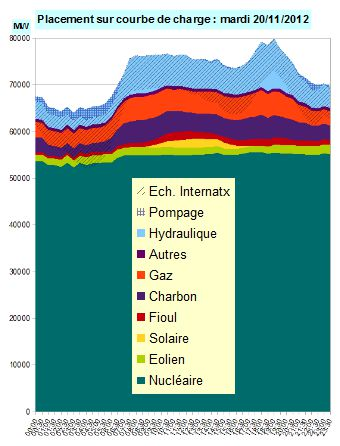
\includegraphics[width=0.5\textwidth]{images/problematique/ccharge.jpg}
 \end{center}
 \caption{Placement du type d'énergie sollicitée sur la courbe de charge française du mardi 20 novembre 2012 (à remplacer par une plus belle/récente)(source RTE)}
 \label{fig:courbeCharge}
\end{figure}

Ces pics sont amenés à connaître une intensification significative avec l'émergence de nouveaux usages de consommation dont, notamment, la mobilité électrique. France, les pouvoirs publics misent sur deux millions de véhicules électriques en circulation en 2020. L'impacte de ces véhicules sur l'équilibre entre l'offre et la demande n'est pas négligeable. En effet, la recharge complète d'un véhicule électrique ayant 150 km d'autonomie est équivalente en terme d'appel de puissance à~:
\begin{itemize}
\item un chauffe-eau si la recharge s'effectue en 8~h (recharge normale)~;
\item un immeuble si la recharge s'effectue en 1~h (recharge accélérée)~;
\item un quartier urbain si la recharge s'effectue en 3~min (recharge rapide).
\end{itemize}



\subsection{Architecture Smart Grids : vers des réseaux électriques flexibles et communicants}

t législaIncitations tarifaires -> pilotage par la demande (effacement)  et
Objectifs environnementaux facteur 4 -> déploiement des ENR -> intermittante, injecte aussi de l'énergie.
nouveaux usages


Infrastructure électriques (ligne, transformateur, centrales de production)
Outils additionnels
Moyens de télécommunication (CPL, 3G, radio, ...)
Technologie de l'information pour automatiser le traitement des informations, contrôler à distance les composants électriques 

Rendre les réseaux électriques intelligents consiste donc en grande partie à les instrumenter pour les rendre communicants.

\begin{figure}[!htbp]
 \begin{center}
  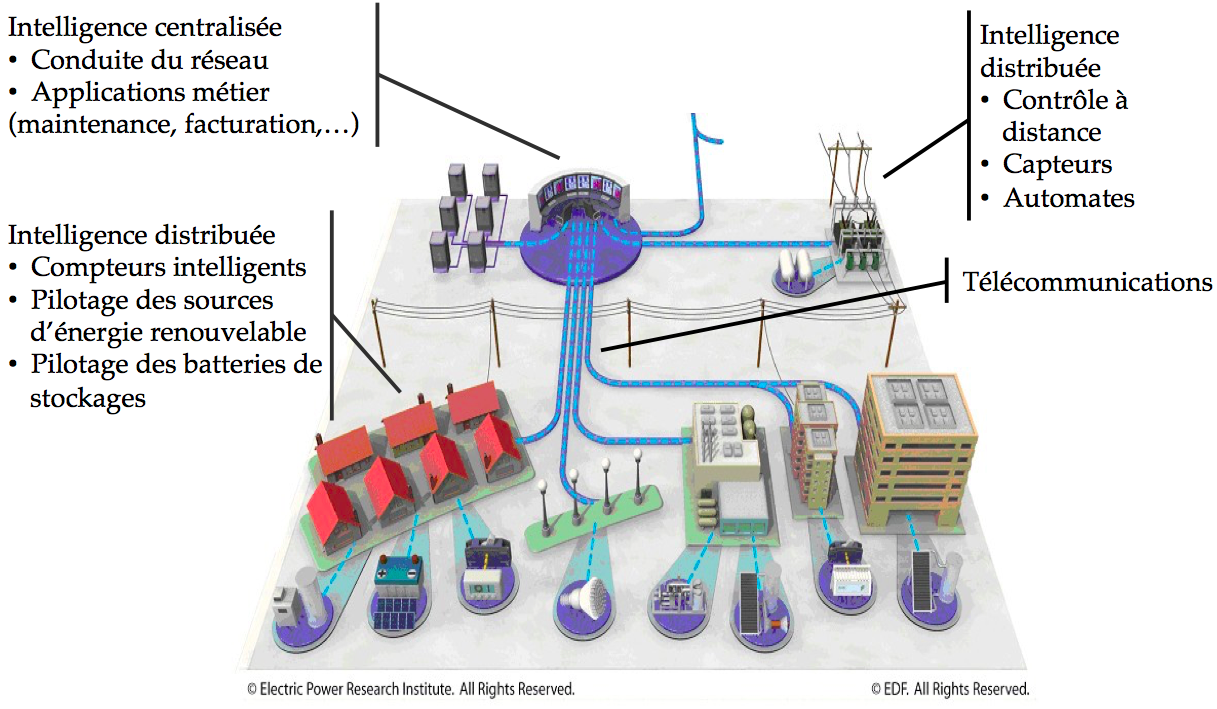
\includegraphics[width=1\textwidth]{images/problematique/archiSmartgrids.png}
 \end{center}
 \caption{Architecture d'un Smart Grid pour la  de l'électricité \protect\cite{favre2006ingenierie}}
 \label{fig:archismartgrids}
\end{figure}






%En effet, la libéralisation du marché de l'électricité exige que le consommateur ait une connaissance en temps réel de l'évolution tarifaire horaire de l'électricité et qu'il puisse même choisir d'injecter sa propre propre production d'énergie sur le réseau.

\section{Impact des Smart Grids sur les SI et l'AE}

Un Smart Grid est un réseau électrique intelligent permettant d'optimiser la production, la distribution et la consommation d'électricité grâce à l'introduction des Technologies de l'Information et de la Communication (TIC) sur le réseau électrique \footnote{www.smartgrids-cre.fr}.

Les compagnies d'électricité doivent faire évoluer leur Systèmes d'Information (SI) car les Smart Grids apportent, par essence, de profonds changements au niveau des SI qui les pilotent  : nouveaux flux d'information provenant du réseau électrique, entrée en jeu de nouveaux acteurs tels que les producteurs décentralisés (éolien, photovoltaïque), nouveaux équipements communicants comme le compteur Linky \footnote{www.erdf.fr/Linky}, nécessaire conformité aux nouvelles réglementations et directives européennes \footnote{www.horizon2020.gouv.fr}, nouveaux usages (véhicule électrique, maison connectée). 

Les Smart Grids impliquent un changement de paradigme que les compagnies d'électricité doivent pleinement intégrer dans leur stratégies de développement en envisageant de nouveaux modèles métier et de nouveaux partenaires, tout en tenant compte des exigences du marché et du législateur et de l'émergence de nouvelles technologies. 

Une étude américaine, menée par IBM, CISCO, EPRI et South Carolina Edison, fait état de cinq thèmes stratégiques clé pour l'implémentation des Smart Grids:
\begin{itemize}
\item Permettre au consommateur de contrôler sa consommation d'énergie et de réduire son emprunte carbone en utilisant des équipement intelligents et des véhicules électriques et en produisant de l'énergie renouvelable à domicile.
\item Améliorer la sécurité et la productivité des employés en mettant à leur disposition des outils performants pour le contrôle à distance, des équipements de protection et des applications mobiles par exemple.
\item Intégrer des sources d'énergie renouvelables distribuées sur le réseau en assurant la protection des équipements électriques, le stockage de l'énergie et la stabilité du réseau.
\item Améliorer l'efficience et la résilience du réseau à travers les systèmes de mesure en temps réel, l'analyse et le contrôle à distance.

%%FB Ce denier point est peut-être une conséquence de l'informatisation qui est nécessaire pour les points précédents (à cause des constantes de temps, du grand nombre de parties prenantes etc.)
\item Fournir les informations et la connectivité nécessaires par le développement d'une infrastructure TIC.
\end{itemize}

Les compagnies d'électricité élaborent souvent différents scénarios de stratégies possibles pour répondre aux enjeux Smart Grid. Mais la prise de décision n'est pas aisée au vue de la complexité des Smart Grids et de la forte interdépendance de composants tels que les cadres de régulation, les consommateurs, les marchés de l'énergie, les technologies en constante évolution). 

%%FB Un peu rapide le "aussi"
%%FB Dire que les 4 1ers points rendent nécessaire l'automatisation des actions et du traitement de l'information, d'où le 5e point, et d'où l'impact des choix stratégiques sur le SI.
Aussi, le choix d'une stratégie impacte-t-il directement le SI. Néanmoins, les processus Smart Grid étant fortement automatisés, la mise en œuvre effective de cette stratégie dépend du SI qui l'exécute.
% et des ressources disponibles (humaines, financières, techniques) ce qui amène donc les parties prenantes à reconsidérer leur choix stratégique.

La question soulevée par ce contexte industriel à laquelle nous nous intéressons est la suivante : \textbf{Comment évaluer une stratégie de développement d'un Smart Grid à travers sa déclinaison au niveau du SI ?}

Évaluer la déclinaison d'une stratégie au niveau du SI oblige à prendre en compte l'architecture globale de la compagnie. %%FB à justifier
Cette activité est connue sous le nom d'Architecture d'Entreprise. En effet, \cite{ross2006enterprise} considèrent que l'architecture d'entreprise offre «~une vision générale de comment une compagnie va mettre en \oe{}uvre sa stratégie~». 

L'exécution effective d'une stratégie est cependant confrontée à des barrières de communication au sein de l'organisation \cite{vcater2010factors}. Le recours à l'architecture d'entreprise est d'autant plus justifié qu'elle représente un outil pour la transmission des objectifs stratégiques à tous les niveaux hiérarchiques de l'organisation en question \cite{kappelman2008enterprise}. 

L'architecture d'entreprise offre une vision globale et transverse de l'entreprise \cite{zachman1987framework}  permettant d'aligner efficacement les intérêts des acteurs impliqués dans l'implémentation des Smart Grids tels que les experts métier, les conseillers stratégiques, les experts environnementaux, les experts en normalisation \cite{buckl2010conceptual}. Le recours à l'architecture d'entreprise est ainsi pleinement justifié.

Les Smart Grids sont, par essence, des systèmes très  dynamiques et complexes \cite{monti_power_2010}. La déclinaison d'une stratégie Smart Grid au niveau du SI de la compagnie engendre ainsi des systèmes dynamiques au comportements complexes. \cite{borshchev2004system} affirme que le seul moyen d'adresser cette complexité est  de simuler ces systèmes. La simulation est une technique connue pour valider ou critiquer la conception d'un système dès les premières étapes de son cycle de développement. Les acteurs impliqués dans l'implémentation des Smart Grids acquièrent, par la  simulation, une connaissance approfondie et directe des modèles créés pour valider ou critiquer un choix stratégique.

Néanmoins, les approches d'architecture d'entreprise se focalisent souvent sur des aspects statiques et structurels tels que les interconnexions entre les différentes applications métier \cite{buckl2008towards}. Les modèles issus de ces approches sont alors utilisés exclusivement à des fins de documentation et de communication entre parties prenantes \cite{kulkarni2013modelling}. 

Notre problématique de recherche émerge de cet état de fait, nous la résumons dans la question suivante :
\textbf{Quels critères doivent satisfaire les modèles issus de l'architecture d'entreprise pour permettre, par la simulation, d'évaluer la stratégie de l'entreprise en question~?}
     
